\documentclass[11pt]{article}
\usepackage[margin=0.8in]{geometry}
\usepackage{graphicx}
\usepackage{amsmath}
\usepackage{hyperref}
\title{Weighted N6 exponent: formal scaling boundary}
\author{aburan28/crypto research packet}
\date{25 October 2026}
\begin{document}
\maketitle

The published genus-2 complete-law article defines a weighted coordinate
action in Section 4 and printed affine doubling coefficients in Eq.~(7).
The pinned author Magma file assigns \texttt{WW1:=W1\string^2} and uses
\texttt{WW1} in its \texttt{N6} assignment. Thus the author code and frozen
Rust runtime both use $W^2$. The earlier report mistook the alias
\texttt{WW1} for \texttt{W1}. The retained $p=739$ regression instead
compares production $W^2$ with a synthetic $W^1$ mutation; only that
mutation differs from independent Cantor. The prior author-code discrepancy
claim is withdrawn. This packet proves the coordinate-scaling distinction,
not complete Jacobian addition.

Under $(S,T,W)\mapsto(\mu S,\mu T,\mu W)$ with $Q,R,Z$ fixed, the represented
affine divisor is unchanged. Put $N1=QS-T$, $N2=RS$,
$N5=S^2-HW^2$ and $N6=DW^2$. Then both
$AA=N1\cdot N5-N2\cdot N6$ and $CC=S\cdot N5-T\cdot N6$
scale by $\mu^3$. If the synthetic mutation $N6=DW$ is used instead, the exact defects are
$\mu^2(\mu-1)RSDW$ for $AA$ and $\mu^2(\mu-1)TDW$ for $CC$.
Four universal polynomial identities and a concrete integer counterexample
were checked by Lean 4.34.1/Mathlib. The axiom audit lists only
\texttt{propext}, \texttt{Classical.choice}, and \texttt{Quot.sound}.
The four native identity certificates are
\texttt{IDC1h92ee5de5110623fd}, \texttt{IDC1h7679e312ee733fcb},
\texttt{IDC1h87fbf5497ad4d6e0}, and \texttt{IDC1he881917e142d1cb5};
each passed 32 sealed and 32 checker-chosen points.

\begin{figure}[h]
\centering
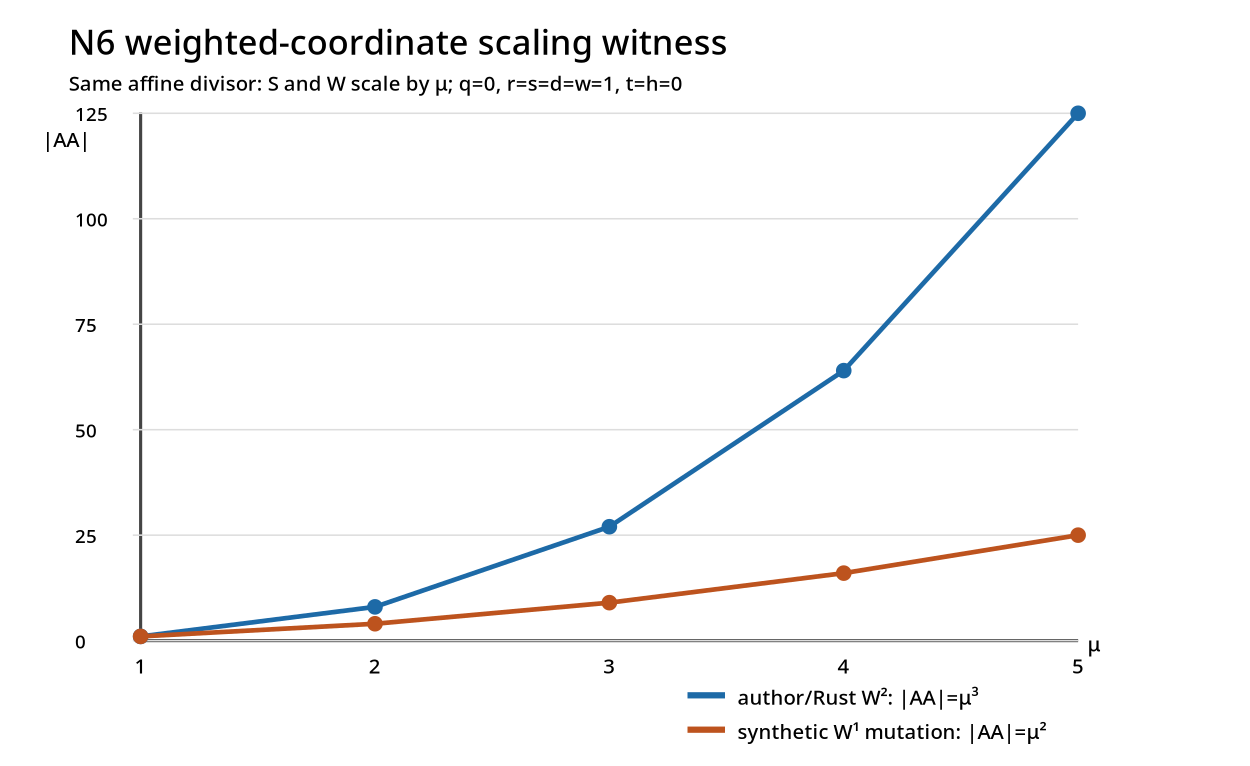
\includegraphics[width=0.77\textwidth]{scaling.png}
\caption{Exact integer illustration from \texttt{scaling.csv}: $Q=T=H=0$,
$R=S=D=W=1$. At $\mu=3$, the same affine input yields $AA=-27$ for $W^2$
and $AA=-9$ for the synthetic $W^1$ mutation. This is a scaling witness, not a cost graph.}
\end{figure}

The frozen Lean file has an incorrect historical author-source comment.
It remains byte-identical because its proof certificates bind its digest;
the source correction beside this report supersedes that comment and proves
that weighted $A,B,C$ reduce to the article's affine Eq.~(7).

The earlier full 1,260-target operation-price ratios are unchanged:
wrapper/rho $3.793783$ and retained-state/rho $4.179297$ at the representative
cell. The Rust-to-Lean semantic correspondence, concrete smooth-curve/Mumford/
$\operatorname{Pic}^0$ bridge, and independent mathematical review remain open.

Sources: \href{https://link.springer.com/article/10.1007/s13389-024-00351-7}{published article}
and \href{https://github.com/ozbayelif/jac-on-jac/blob/ec98e115ed359c8b7facf559eb0d9f240703f6f5/jac-on-jac.m}{pinned author code}.
\end{document}
